\documentclass[aps,preprint,nofootinbib,floatfix]{revtex4-1}

%\usepackage{cite}
\usepackage[pdftex]{graphicx}
\graphicspath{{./figures/}}
%\graphicspath{{./}}
\usepackage{amsmath,amssymb,amsfonts,amsthm,amscd,bm}
\usepackage{bbm}
\usepackage{algorithm}
\usepackage{algorithmic}
%\usepackage{epstopdf}
%\usepackage{fixltx2e}
%\usepackage{stfloats}

\hyphenation{op-tical net-works semi-conduc-tor}

\newtheorem{theorem}{Theorem}
\newtheorem{definition}[theorem]{Definition}
\newtheorem{assumption}[theorem]{Assumption}
\newtheorem{lemma}[theorem]{Lemma}
\newtheorem{corollary}[theorem]{Corollary}
\newtheorem{proposition}[theorem]{Proposition}
\newtheorem{conjecture}[theorem]{Conjecture}
\newtheorem{remark}[theorem]{Remark}
\newtheorem{example}{Example}

%% our definitions %%%%%%%%%%%%%%%%%%%%%%%%%%%%%%%%%%%%%%%%%%%%%%%%%%%%%%%%%%%%
\DeclareMathOperator{\aff}{aff}
\DeclareMathOperator{\st}{s.t.}
\DeclareMathOperator{\LC}{LC}
\DeclareMathOperator{\affnot}{aff_0}
\DeclareMathOperator{\conv}{conv}
\DeclareMathOperator{\relint}{relint}
\DeclareMathOperator{\vol}{vol}
\DeclareMathOperator{\range}{range}
\DeclareMathOperator{\image}{im}
\DeclareMathOperator{\nullspace}{null}
\DeclareMathOperator{\area}{area}
\DeclareMathOperator{\vspan}{span}
\DeclareMathOperator{\id}{Id}
\DeclareMathOperator{\cond}{cond}
\DeclareMathOperator{\prox}{prox}
\DeclareMathOperator*{\argmax}{arg\,max}
\DeclareMathOperator*{\argmin}{arg\,min}
\DeclareMathOperator*{\minimize}{minimize}
\DeclareMathOperator{\diag}{diag}
\DeclareMathOperator{\Tr}{Tr}

\graphicspath{{figs/}}

\begin{document}

\title{Discussion about $k$-Means and $1D$ Random Projections}

\author{Guilherme Fran\c ca}
%\email{guifranca@gmail.com}
%\affiliation{Johns Hopkins University, Center for Imaging Science}

\maketitle

\section{Procedure}

Given data $X=\{ x_i \}_{i=1}^{n}$, where $x_i \in \mathbb{R}^{D}$, 
and the number of clusters $k$, we perform the following experiments:
\begin{enumerate}
\item Run $k$-means$++$ 
on the original data space. This is the column named 
``$k$-means'' in the following tables.
\item Use PCA to 
project the data in the first principal component, 
$Y=\{ y_i \}_{i=1}^n$ where $y_i = u_{1}\cdot x_i \in \mathbb{R}$, then
apply $k$-means in this $1$-dimensional space. This is the column named
``PCA'' in the following tables.
\item We randomly project the data in one dimension by picking a vector
$w$ such that $w_i \sim \mathcal{N}(0,1)$ and normalize it $\| w \|=1$.
Thus $Y = \{y_i\}_{i=1}^n $ where $y_i = w\cdot x_i \in \mathbb{R}$. 
We apply $k$-means in this randomly projected
$1$-dimensional space. We do this several times and pick the best answer.
This is the column named ``Random'' in the fllowing tables.
\end{enumerate}

The evaluation of the clustering procedure 
will be based on the true labels by the following quantity, called
accuracy:
\begin{equation}
\label{eq:accuracy}
a(z,\hat{z}) = 
\dfrac{1}{n}\sum_{i=1}^{n} \mathbbm{1}\left(z_i = \pi(\hat{z}_i) \right)
\end{equation}
where $z$ is an $n$-dimensional vector containing the true labels, entry
$z_i$ corresponds to point $x_i$, and $\hat{z}$ is the estimated labels
through the clustering procedure. $\pi$ is a permutation of the labels.
Thus the above formula gives $1$ if all points were correctly classified and
$0$ if all points were wrongly classified. In a two class problem with
the same number of points, $a=1/2$ corresponds to picking the points in each
cluster at random. This quantity $a$ is the number shown in the following tables.

\paragraph*{How to choose the best answer for random projections?}
Consider $k$-means objective function
\begin{equation}
\label{eq:J}
J(X) = \dfrac{1}{2} \sum_{j=1}^k \sum_{x \in \mathcal{C}_j} \| x - m_j \|^2,
\qquad
m_j = \dfrac{1}{n_j}\sum_{x\in\mathcal{C}_j} x.
\end{equation}
Above $m_j$ is the center
of cluster $\mathcal{C}_j$, and 
$n_j$ is the number of elements in cluster $\mathcal{C}_j$. $k$-means
algorithm solves the problem $\min_{\{C_j\}} J(X)$. 

One might think
that a good criteria to choose the best answer is to pick the minimum $J(Y)$
computed in the $1D$ randomly projected space. This doesn't work because
each random projection gives different values for the data $Y$ which in general
does not preserve the structure in the original
distribution. For instance, considering two random projections yielding
$Y_1$ and $Y_2$. It can happen that the clustering on $Y_2$ gives a better
accuracy than the clustering on $Y_1$ and even though $J(Y_1) < J(Y_2)$.
So we are really comparing apples and bananas here.

Another approach would be to cluster on $Y$ yielding labels $\hat{z}$, then
compute $J(X)$ based on these labels, and pick the smallest $J(X)$  computed
on the original data. This only works in case where $k$-means in the original
space itself provides a good answer. For cases where $k$-means is problematic,
e.g. the data are not spherical gaussians, then $J(X)$ itself is not a good
function to detect the clustering. This happens for parallel cigars in the
example below.

Thus if one still desires to follow this approach, a good function which
does not depend on the true labels must be chosen. I tried to use the energy
function for this, and still didn't quite work. Also, observe that the 
energy function on the original space is expensive to compute, 
$O(n^2)$.

In the following experiments I will \emph{cheat} and use \eqref{eq:accuracy}
to pick the best answer. The purpose of this is to see if the ``truth'' can
be captured by random projections.

\section{Experiments}

In the first experiment shown in Fig.~\ref{fig:2d_gauss_sep} we choose
two well separated gaussians in $2D$. All of these procedures give good
results.

\begin{figure}
\begin{minipage}{.49\textwidth}
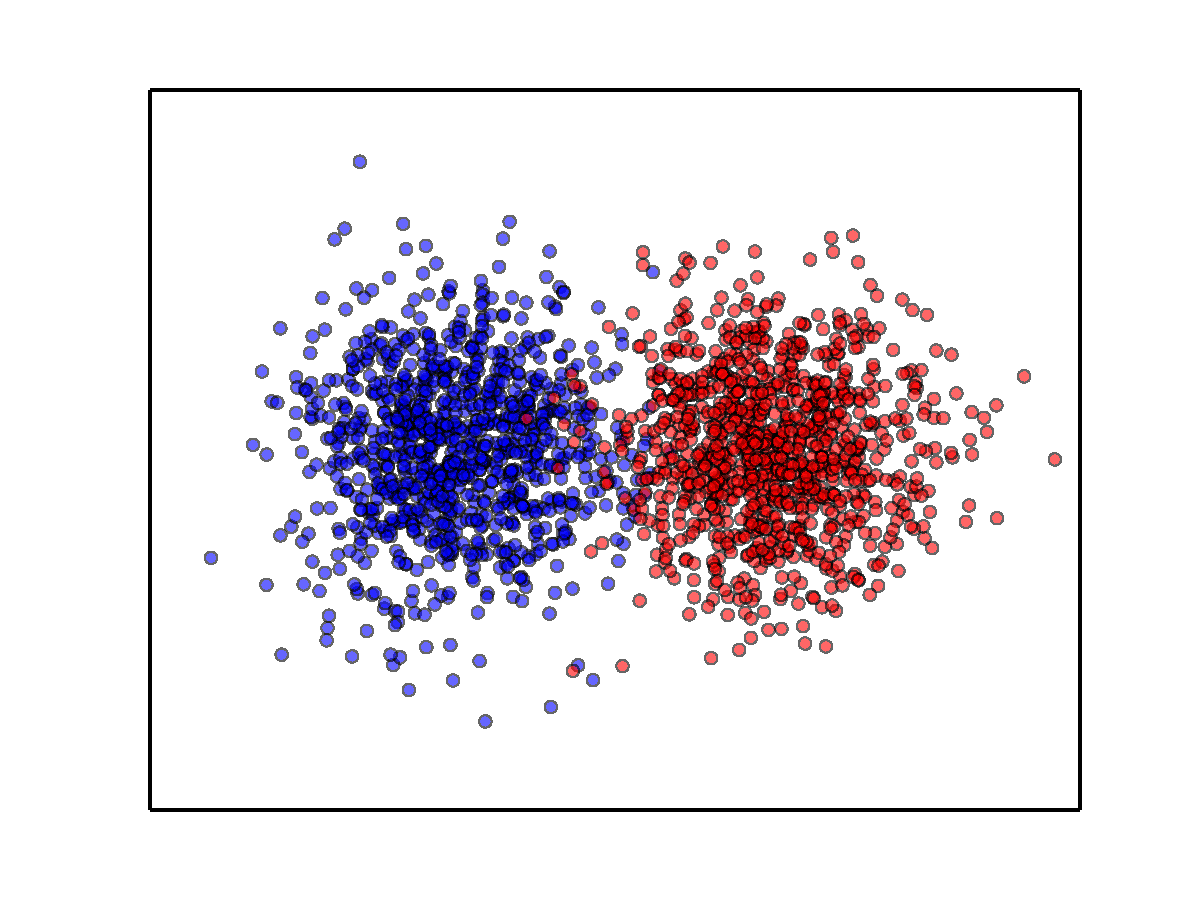
\includegraphics[scale=.45]{2d_gauss_separate.pdf}
\end{minipage}
\begin{minipage}{.49\textwidth}
\begin{tabular}{ l  l  l }
\hline
$k$-means~~ & PCA~~~~ & Random \\
\hline
0.9735 & 0.9735 & 0.9755 \\
0.978 & 0.978 & 0.979 \\
0.977 &  0.9775 & 0.978 \\
\hline
\end{tabular}
\end{minipage}
\caption{\label{fig:2d_gauss_sep}
We have $x \sim \tfrac{1}{2}\left( \mathcal{N}(\mu_1, I) +
\mathcal{N}(\mu_2, I)\right)$ where $\mu_1 = (0,0)^T$ and $\mu_2=(4,0)^T$,
and $1000$ points on each cluster. We run the experiment three times.
}
\end{figure}

In the experiment of Fig.~\ref{fig:cigar}, still in $2D$, we choose
parallel cigars. Both $k$-means and PCA cannot perform well, however random
projections can do well. This is not surprising because this data
can be linearly separable in $1D$. After many tries random projections will
find the correct line. Probably, LDA can perform as well on this example.

\begin{figure}
\begin{minipage}{.49\textwidth}
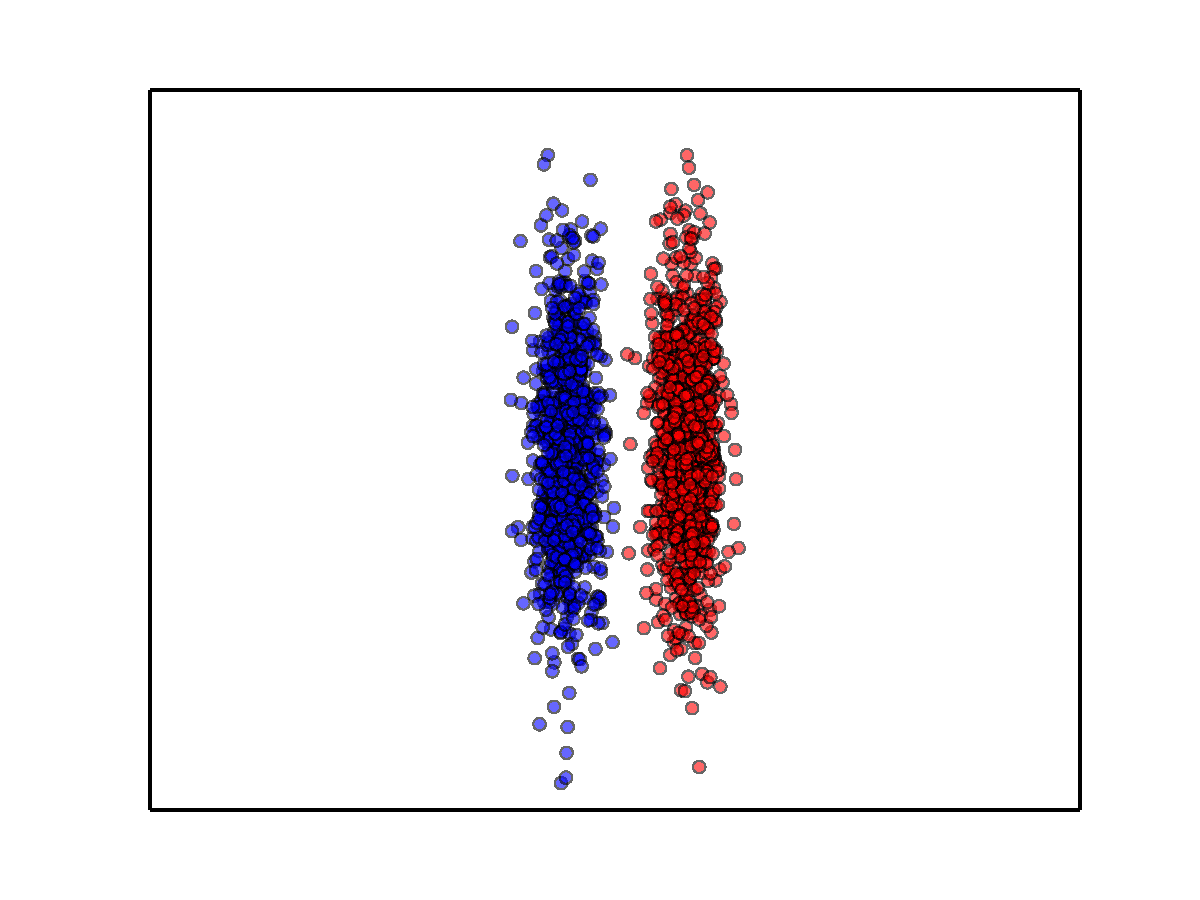
\includegraphics[scale=.45]{2d_cigar.pdf}
\end{minipage}
\begin{minipage}{.49\textwidth}
\begin{tabular}{  l  l  l }
\hline
$k$-means~~ & PCA~~~~ & Random \\
\hline
0.501 & 0.5075 & 0.9995 \\
0.522 & 0.515 & 1.0 \\
0.505 & 0.5055 & 0.9995 \\
\hline
\end{tabular}
\end{minipage}
\caption{\label{fig:cigar}
We have $x \sim \tfrac{1}{2}\left( \mathcal{N}(\mu_1, \Sigma) +
\mathcal{N}(\mu_2, \Sigma)\right)$ where $\mu_1 = (0,0)^T$, $\mu_2=(5,0)^T$,
and $\Sigma = \left( \begin{smallmatrix} 1/2 & 0 \\ 0 & 15 \end{smallmatrix}
\right)$,
and $1000$ points on each cluster. We run the experiment three times.
}
\end{figure}

In the experiment of Fig.~\ref{fig:highd} we increase the number of
dimensions of the gaussian distributions. Both $k$-means and PCA perform well
if the dimension is not too high, while $1D$ random projections provide
poor results. This is also expected since randomly projecting high dimensional
data in a very low dimensional space practically destroy any information
about the original distribution.

\begin{figure}
\begin{minipage}{.49\textwidth}
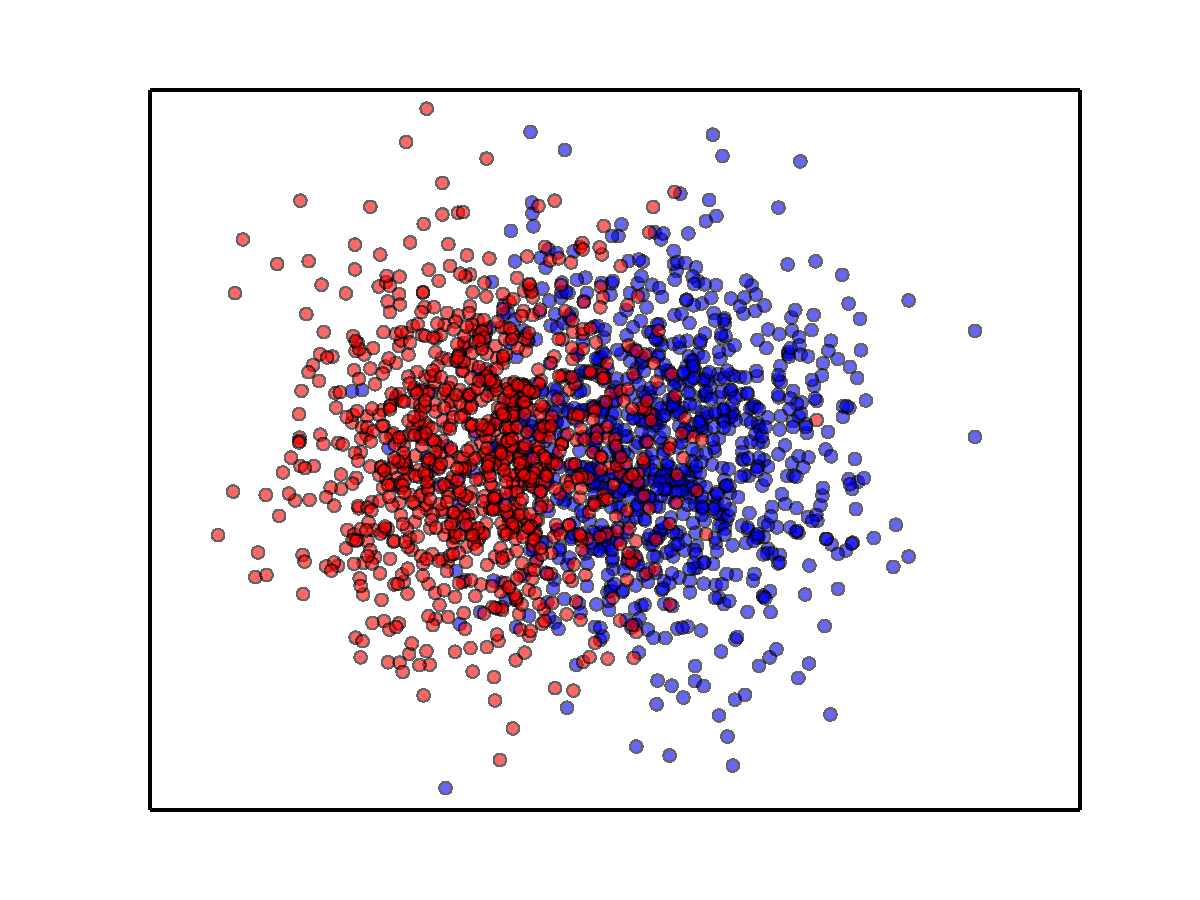
\includegraphics[scale=.45]{30d_gauss.pdf}
\end{minipage}
\begin{minipage}{.49\textwidth}
\renewcommand*{\arraystretch}{.3}
\begin{tabular}{ l l l l }
\hline
$D$ & $k$-means~~ & PCA~~~~  & Random \\
\hline
5 & 0.84 & 0.8415 & 0.841 \\
10 & 0.844 & 0.846 & 0.7985 \\
15 & 0.8325 & 0.8365 & 0.7465 \\
20 & 0.846 & 0.85 & 0.764 \\
25 & 0.8555 & 0.8505 & 0.714 \\
30 & 0.825 & 0.8225 & 0.728 \\
50 & 0.8485 & 0.8465 & 0.6775 \\
100 & 0.832 & 0.8325 & 0.644 \\
200 & 0.8085 & 0.8145 & 0.592 \\
300 & 0.7645 & 0.794 & 0.5755 \\
500 & 0.6915 & 0.756 & 0.5615 \\
1000 & 0.5075 & 0.6965 & 0.562 \\
2000 & 0.5495 & 0.662 & 0.543 \\
5000 & 0.531 & 0.5135 & 0.539 \\
\hline
\end{tabular}
\end{minipage}
\caption{\label{fig:highd}
High dimensions.
We have $x \sim \tfrac{1}{2}\left( \mathcal{N}(\mu_1, I_D) +
\mathcal{N}(\mu_2, I_D)\right)$ where $\mu_1 = (0,0,\dotsc,0)^T$,
$\mu_2=(1,0,\dots,0)^T$,
and $1000$ points on each cluster. We show the two principal components
of the data in the plot above.
}
\end{figure}

\end{document}
